\documentclass{article}

\usepackage{tikz}

\begin{document}
\begin{figure}[h!]
  \begin{center}
    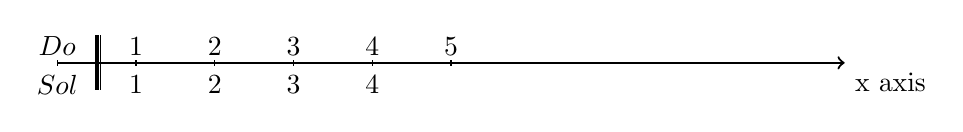
\begin{tikzpicture}
        \draw[thick,->] (0,0) -- (10,0) node[anchor=north west] {x axis}; % main ligne
        \draw (0cm, 1pt) -- (0cm, -1pt) node [anchor=south] {$Do$};  % init ligne Do
        \draw (0cm, 1pt) -- (0cm, -1pt) node [anchor=north] {$Sol$};  % init ligne Sol
        \draw [line width=0.5mm ] (0.5cm, 10pt) -- (0.5cm, -10pt) node {};
        \draw (0.55cm, 10pt) -- (0.55cm, -10pt) node {};
        \draw (5cm, 1pt) -- (5cm, -1pt) node [anchor=south] {$5$};
          \foreach \x in {1,2,3,4}
            \draw (\x cm,1pt) -- (\x cm,-1pt) node[anchor=south] {$\x$};
          \foreach \x in {1,2,3,4}
            \draw (\x cm,1pt) -- (\x cm,-1pt) node[anchor=north] {$\x$};
    \end{tikzpicture}
    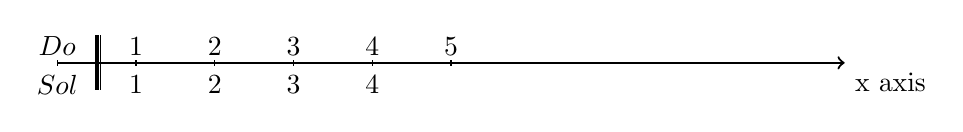
\begin{tikzpicture}
        \draw[thick,->] (0,0) -- (10,0) node[anchor=north west] {x axis}; % main ligne
        \draw (0cm, 1pt) -- (0cm, -1pt) node [anchor=south] {$Do$};  % init ligne Do
        \draw (0cm, 1pt) -- (0cm, -1pt) node [anchor=north] {$Sol$};  % init ligne Sol
        \draw [line width=0.5mm ] (0.5cm, 10pt) -- (0.5cm, -10pt) node {};
        \draw (0.55cm, 10pt) -- (0.55cm, -10pt) node {};
        \draw (5cm, 1pt) -- (5cm, -1pt) node [anchor=south] {$5$};
        \foreach \x in {1,2,3,4}
            \draw (\x cm,1pt) -- (\x cm,-1pt) node[anchor=south] {$\x$};
        \foreach \x in {1,2,3,4}
            \draw (\x cm,1pt) -- (\x cm,-1pt) node[anchor=north] {$\x$};
    \end{tikzpicture}
    \caption{Example graphic made with tikz.}
  \end{center}
\end{figure}
\end{document}
